\documentclass[10pt,twocolumn,letterpaper]{article}

\usepackage{cvpr}
\usepackage{times}
\usepackage{epsfig}
\usepackage{graphicx}
\usepackage{amsmath}
\usepackage{amssymb}

% Include other packages here, before hyperref.

\graphicspath{ {./figures} }

% If you comment hyperref and then uncomment it, you should delete
% egpaper.aux before re-running latex.  (Or just hit 'q' on the first latex
% run, let it finish, and you should be clear).
\usepackage[breaklinks=true,bookmarks=false]{hyperref}

\cvprfinalcopy % *** Uncomment this line for the final submission

\def\cvprPaperID{****} % *** Enter the CVPR Paper ID here
\def\httilde{\mbox{\tt\raisebox{-.5ex}{\symbol{126}}}}

% Pages are numbered in submission mode, and unnumbered in camera-ready
%\ifcvprfinal\pagestyle{empty}\fi
\setcounter{page}{1}
\begin{document}

%%%%%%%%% TITLE
\title{An Efficient Model for Traffic Sign Recognition}

\author{Aidan Chaplin\\
Georgia Institute of Technology\\
{\tt\small achaplin3@gatech.edu}
% For a paper whose authors are all at the same institution,
% omit the following lines up until the closing ``}''.
% Additional authors and addresses can be added with ``\and'',
% just like the second author.
% To save space, use either the email address or home page, not both
\and
Hoa Luu\\
Georgia Institute of Technology\\
{\tt\small hluu8@gatech.edu}
}

\maketitle
%\thispagestyle{empty}

%%%%%%%%% ABSTRACT
\begin{abstract}
   Computer vision is beset with models that deliver high performance, but at the cost of having tens or hundreds of millions of parameters. Many models require a large amount of data and compute power to train, and necessitate the use of additional optimization libraries for efficient inference. We show that, for traffic sign recognition, it is possible to create a model with similar accuracy to extant solutions, but using a fraction of the parameters. 
\end{abstract}

%%%%%%%%% BODY TEXT
\section{Introduction}
Traffic signs and roads are intrinsically linked; the demanding and isolated nature of driving requiring a method of communication that is both efficient and nonverbal. Traffic signs can provide guidance, warn drivers of hazards, remove uncertainty, and prepare drivers for the road ahead. Pedestrians can  make use of traffic signs, too -- much of what is communicated to drivers is relevant to pedestrians, and can inform their travel decisions as well. 

\subsection{Motivation}
We design a lightweight, high-accuracy model that  can recognize these traffic signs. Avoiding complex, state-of-the-art deep  learning methods, we instead opt for the fundamentals of computer vision  to see how far they can be pushed. 

Our intention is not that this model is  used in performance-critical contexts, but rather in resource-critical ones -- we  deliver comparable performance at a fraction of the cost. Additionally, the  simplicity of the model means that fine-tuning the network for use with  other traffic signs is just as simple. 

\subsection{Dataset}
For this task, we made use of the German Traffic Sign Recognition Benchmark  (GTSRB) \cite{Stallkamp2012}. The dataset is publicly available online, and is commonly used for computer vision evaluation. It was released originally by the 2011  International Joint Conference on Neural Networks under the Creative Commons 0 license, placing the dataset "as completely as possible in the public domain" \cite{creative-commons-2017}. 

\begin{figure}[h]
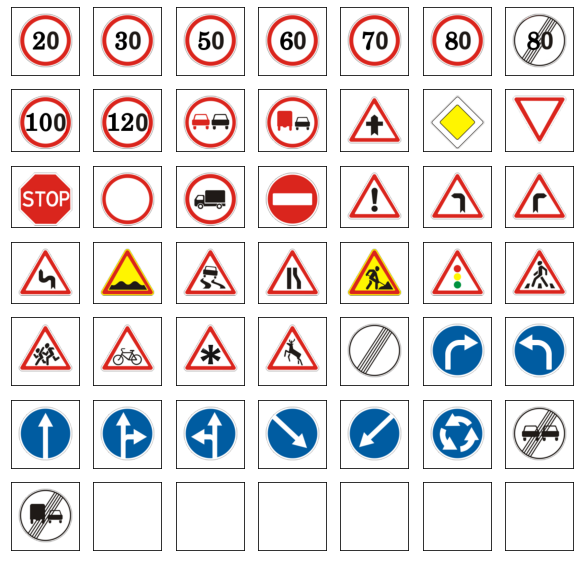
\includegraphics[width=7cm]{class-examples}
\centering
\caption{Prototypes for each of the GTSRB's 43 classes}
\end{figure}

The dataset consists of approximately 50,000 images of 43 types of German traffic signs, cropped to show only the sign itself but otherwise unaltered. They are  labeled with numbers 1 to 43 inclusive and contain no identifying or otherwise sensitive data. In other words, the GTSR Benchmark is a good benchmark. 

\subsection{Current Solutions} 
Most state-of-the-art solutions borrow from other sub-disciplines of deep  learning, utilizing techniques such as transformers and self-attention.  Indeed, one solution boasting 99.8\% accuracy incorporated both spatial transformers and a modified version of Google's inception module \cite{https://doi.org/10.48550/arxiv.1511.02992}. Others  use either very large CNNs or a committee of CNNs -- a deep learning  construct that takes the idea of a random forest and applies it to CNNs -- to achieve a similarly high level of accuracy \cite{https://doi.org/10.48550/arxiv.1511.02992}. 
 
However, a constant theme between all high-performing networks is  complexity. The aforementioned committee of CNNs had approximately  90 million parameters, and required both 25 concurrent networks and "dataset dependent handcrafted augmentations" \cite{https://doi.org/10.48550/arxiv.1511.02992}. The modified inception architecture seems almost slim by comparison, weighing in  at 10.5 million parameters \cite{https://doi.org/10.48550/arxiv.1511.02992}. Neither solution, though, could be considered accessible. Fine-tuning alone would take considerable compute resources, not to mention training from scratch. 

\section{Data Exploration and Preparation}
As with any good machine learning undertaking, our first step was to examine the data, see if there exist any glaring inadequacies that we could fix before beginning training. We pinpointed two key problems, that of class imbalance and that of insufficient contrast, and fixed them using common methods before beginning training. 

\subsection{Class Imbalance}
Upon plotting the number of classes against the total number of their respective examples, a clear imbalance can be seen -- some classes, such as 0 and 19, have  around 300 examples, while others have 10 times as many. 

\begin{figure}[h]
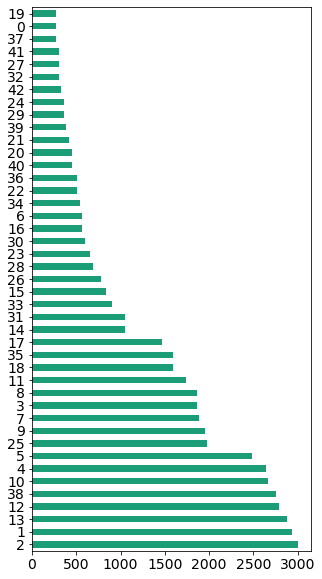
\includegraphics[width=6.75cm]{class-distribution}
\centering
\caption{Class distributions for each of GTSRB's 43 classes}
\end{figure}

We combat this skew in two ways: first, we use several kinds of data augmentation at training time. Specifically, we allow small amounts of random rotations, random shears,  and random shifts along the x- and y-axes. This helps the smaller classes seem to have more variance to the model, allowing it to better generalize from the smaller number of samples. 

Secondly, we weight the classes by their distribution at training time. For each  class $c$, the weight $w_c$ of $c$ can be found via 

\begin{equation}
    c_w=\frac{\max_{c\in C}|c|{}}{|c|}
\end{equation}

So, for example, if class $c'$ has $1|c'|$ examples, and the maximum number of examples
is $2|c'|$, then $w_c'=2$, leading to $c'$ being seen twice as many times. 

\subsection{Insufficient Contrast} 

As mentioned, the GTSRB dataset has no preprocessing performed other than crops to the target sign. Because of this, there is a large amount of variance found in the images in terms of both degree of contrast and the overall image brightness. 

As Figure \ref{fig:preclahe} shows, many images are too dark to be seen clearly, and some are either washed out or too bright to be useful. 

\begin{figure}[h]
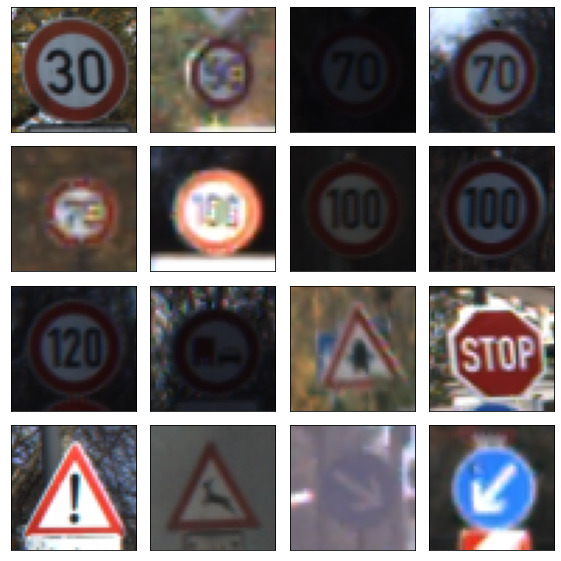
\includegraphics[width=8cm]{example-clahe-before}
\centering
\caption{16 random samples from GTSRB}
\label{fig:preclahe}
\end{figure}

However, by applying a normalization  technique known as contrast-limited adaptive histogram equalization (CLAHE), we were able to drastically improve and homogenize the quality of GTSRB's images. 

As Figure \ref{fig:postclahe} shows, the samples are far more similar after CLAHE than before; the image in the third column of the first row goes from almost completely invisible to almost the same fidelity as its neighbors. 

\begin{figure}[h]
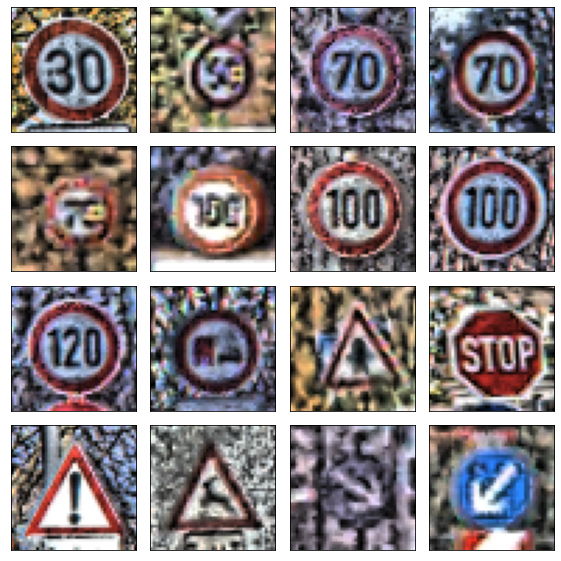
\includegraphics[width=8cm]{example-clahe-after}
\centering
\caption{The same 16 samples from GTSRB after applying CLAHE}
\label{fig:postclahe}
\end{figure}



The first step of CLAHE is to convert the input image to the HSV (Hue, Saturation, Value) color model, to make it easy to change the image's brightness without affecting the other values \cite{clahe}. Then, the image is subdivided into tiles -- a common value is $\frac{1}{8}$ of the image's height by $\frac{1}{8}$ of its width -- to prevent an outlier brightness having too much effect on the resultant image \cite{clahe}. Then, a histogram is calculated for each tile $t$ of the original image based on the image's value (i.e. brightness) \cite{clahe}. 

\begin{figure}[h]
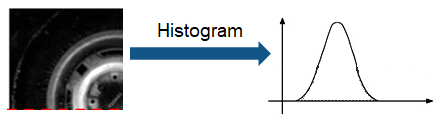
\includegraphics[width=8cm]{clahe-step-1}
\centering
\caption{Calculating an image histogram \cite{clahe}}
\end{figure}

After this, the histogram is clipped at some value in $(0, 1)$. What makes this different from traditional histogram equalization, however, is that the excess is redistributed uniformly to the rest of the image's histogram, as demonstrated by Figure \ref{fig:clahe2} \cite{clahe}. 

\begin{figure}[h]
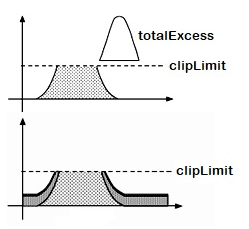
\includegraphics[width=6cm]{clahe-step-2}
\centering
\caption{Clipping and redistribution of excess brightness \cite{clahe}}
\label{fig:clahe2}
\end{figure}

From this resultant histogram, a cumulative distribution function is calculated and used to map and scale the histogram back to the original image. Once this process has been completed for all tiles, the tiles are stitched together using bilinear interpolation, and the final image is obtained. 

\section{Training the Network} 
After exploring the dataset and fixing any problems we could see, the next step was training our network. As we wanted to achieve high accuracy using a simple network of computer vision fundamentals, we started small and built up incrementally. 

\subsection{Frameworks, Libraries, and Other Numbers}
For data exploration and visualization, we used primarily Pandas along with some  scikit-image \cite{scikit-image} functions. Model training was performed via TensorFlow v2.7.0, and accelerated on a Nvidia GeForce RTX 3060 Ti using CUDA v11.4 and cuDNN v8.2.1.32. We also used the scikit-image library to run CLAHE on our images. 

\subsection{Model Architecture}
Since our intent was to create a simple model, it should come as no surprise that  our model is simple. We ended up creating blocks of Conv $\rightarrow$ Conv $\rightarrow$ MaxPool $\rightarrow$ Dropout, and used three of these blocks. The first and second blocks have their inputs zero-padded, while the third block does not. The convolutional layers of the first block learn 16 and 32 filters, then those of the second block learn 32 and 64, and those of the final block learn 64 and 32, respectively. 

After the third block, the output is flattened and passed to a fully connected layer with 64 hidden units, then a dropout layer, and finally to our classification layer with 43 hidden units. Every layer with learnable parameters (so, the fully connected and the convolutional) uses the ReLU activation function, and all dropouts have an activation probability of $0.25$. Our pooling size is (2x2). 

\begin{figure*}
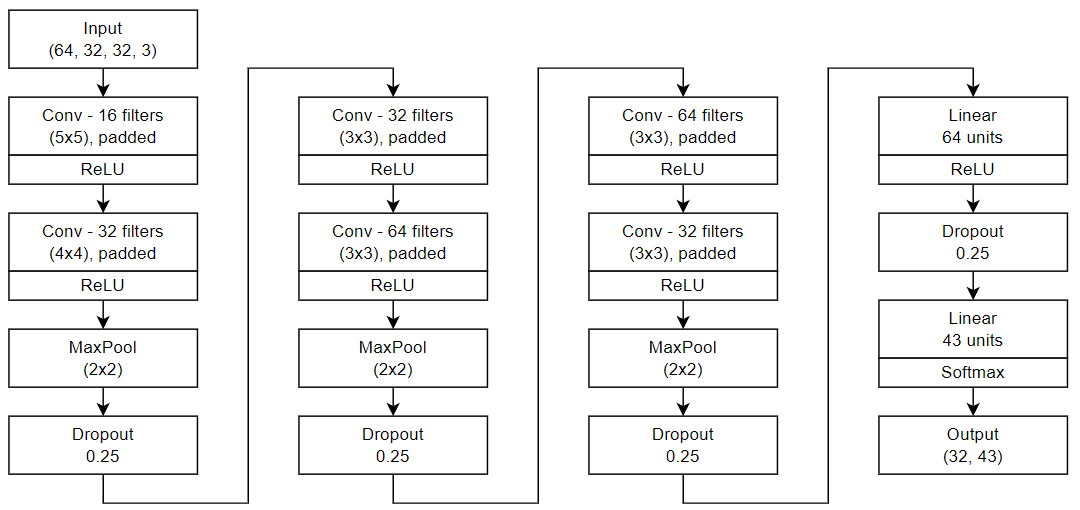
\includegraphics[width=14cm]{model-diagram}
\centering
\caption{Block diagram of our final model }
\label{fig:model}
\end{figure*}

\subsection{Training the Model}
GTSRB comes with pre-split data, with 75\% of the data for training and the remaining 25\% for testing. This split results in 39,209 total images for training, and 12,630 total images for testing. 

Due to the large amount of data, we elected to further split the training data, taking 80\% for training and 20\% for validation, giving us a final training size of 31,368 images, a final validation size of 7,841 images, and a final testing size of 12,630 images. While this does result in a smaller training set, the validation set allowed us to evaluate our model every epoch without risking any data leakage. 

Our data augmentations were all applied lazily at training time, including CLAHE -- we determined that applying this was negligible due to vectorization, and thought it would be better to keep the dataset untouched, in case we later decided to use another normalization method. We used the Keras \texttt{ImageDataGenerator} to handle fetching, batching, and otherwise transforming our images, but other libraries such as \href{https://www.tensorflow.org/guide/data}{\texttt{tf.data}} or \href{https://pytorch.org/data/beta/index.html}{\texttt{torchdata}}. 

Due to GPU memory constraints, we trained with a batch size of 64, and used traditional categorical crossentropy as our loss. Our optimizer was Adam, with a learning rate of 0.001 -- however, if at any point during the training, the validation loss increased or plateaued for more than a few consecutive epochs, the learning rate would be reduced by a value of $0.1$. This allowed us to take advantage of the quick convergence of a higher learning rate, but not lose precision as our loss approached 0. This reduction happened once, at 31 epochs. 

We trained for 38 epochs, and included a callback that would stop training if the validation loss increased or plateaued for several consecutive epochs, but this callback was not used. 

\subsection{Results}

\begin{figure}[h]
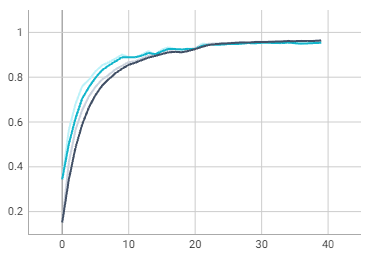
\includegraphics[width=7cm]{epoch-accuracy}
\centering
\caption{Train (dark blue) and validation (light blue) accuracy over 38 epochs}
\label{fig:epochaccuracy}
\end{figure}

As mentioned, we wanted to create our network in a way that optimized for both high accuracy and low parameter count simultaneously. To that end, we have succeeded -- our model achieves 96.11\% accuracy on our test split, with only 103,627 total parameters. This represents a parameter reduction of almost 100\%, but an accuracy reduction of less than 3\%. Being 43x43, our confusion matrix was too large to include here, but no class had a misclassification rate of higher than 7\%. 

\begin{figure}[h]
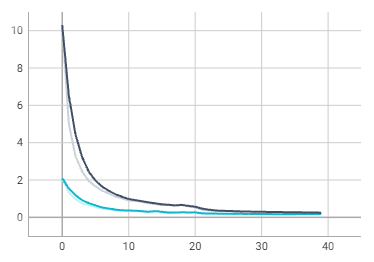
\includegraphics[width=7cm]{epoch-loss}
\centering
\caption{Train (dark blue) and validation (light blue) loss over 38 epochs}
\label{fig:epochloss}
\end{figure}

As the losses in Figure \ref{fig:epochloss} show, our model did not overfit at any point during the training process. The higher training loss than validation loss at the beginning, while unusual, is not unexpected -- it can be explained by our use of dropout at almost every point in the network, intended to combat overfitting. Because of how dropout works, at the beginning of the training process the network will have fewer "good" connections when dropout is active during training compared to when it is not active during validation. 

\section{Conclusion}
We have successfully shown that, for traffic sign recognition, it is very possible to achieve accuracy close to state-of-the-art techniques using only the basics of computer vision and deep learning, affording us comparable performance at a fraction of the cost. We hope that this will both provide a low-cost, portable base for traffic sign recognition around the world, and inspire further research with a similar desire to minimize network parameters. 
%-------------------------------------------------------------------------

{\small
\bibliographystyle{ieee_fullname}
\bibliography{sources}
}

\begin{center}
\begin{tabular}{ |c|c| } 
\hline
Name & Contributions \\
\hline \hline
Aidan & Data wrangling, visualization, preprocessing, model training, paper outlining \& writing\\
\hline
Hoa & Data visualization, model prototyping, training assessment, paper outlining\\
\hline 
\end{tabular}
\end{center}

\end{document}